
\documentclass{studrep}

\RequirePackage{tabularx}
% \RequirePackage{graphicx}

\graphicspath{{pics/}}

% \usepackage{showframe}

% pygmetize
\RequirePackage{minted}
\usemintedstyle{tango} % bw

% \setmainfont{Times New Roman}

\begin{document}
\thispagestyle{empty}
\begin{center}
Министерство науки и высшего образования Российской Федерации

Федеральное государственное бюджетное образовательное учреждение\\ высшего образования

«Иркутский государственный университет»\\
(ФГБОУ ВО «ИГУ»)

Институт математики и информационных технологий

Кафедра информационных технологий
\end{center}

\vfill
\begin{center}
  \textbf{ ВЫПУСКНАЯ КВАЛИФИКАЦИОННАЯ РАБОТА\\
БАКАЛАВРА}
\vspace{1em}

по направлению 02.03.03 -- Математическое обеспечение и администрирование информационных систем

профиль <<общий>>

\vspace{2em}
ТЕМА БОЛЬШИМИ БУКВАМИ

\end{center}
\vfill

\noindent\begin{tabularx}{\textwidth} {
  >{\raggedright\arraybackslash}X
  >{\raggedright}X }
&

Студента 4 курса очного отделения\\
группы 02441-ДБ\\
Фамилия Имя Отчество\\[2em]

Руководитель:\\
к.~т.~н., доцент\\
\underline{\hspace{3cm}} Иванов Иван Иванович\\[2em]

Допущена к защите\\
Зав.каф., к.~т.~н., доцент\\
\underline{\hspace{3cm}} Черкашин Евгений\\ \hspace{3cm} Александрович\\[2em]

\end{tabularx}
\vfill
\begin{center}
  Иркутск -- 2022
\end{center}
\clearpage

\tableofcontents

\chapter*{ВВЕДЕНИЕ}
% TODO: Add contents line
\label{chap:intro}

\chapter{Теоретические основы \ldots}
% Другой пример названия
%\chapter{Математическое обеспечение и технологии разработки ... \ldots}

Согласно \cite{bratko90}

.... база данных (БД) .....

\chapter{Реализация ....}

\section{Скрипт порождения структуры базы данных}
\label{sec:struct-bd}

Начало абзаца


\begin{figure}[htbp]
\begin{center}
\begin{minted}[fontsize=\normalsize]{sql}
CREATE TABLE Persons (
    PersonID int,
    LastName varchar(255),
    FirstName varchar(255),
    Address varchar(255),
    City varchar(255)
);
\end{minted}
\end{center}
\caption{Скрипт SQL для создания таблицы Persons}\label{fig:create-table}
\end{figure}

\begin{lstlisting}[
  caption={Скрипт SQL для создания таблицы Persons},  % Подпись
  captionpos=b,               % Подпись снизу
  basicstyle=\small\ttfamily, % Размер и тип шрифта для представления листинга
  language=SQL
  ]
CREATE TABLE Persons (
    PersonID int,
    LastName varchar(255),
    FirstName varchar(255),
    Address varchar(255),
    City varchar(255)
);
\end{lstlisting}


\chapter{Тестирование программной системы в нагруженной среде}

Разработан набор тестов структуры БД (см.~\ref{sec:struct-bd} на стр.~\pageref{sec:struct-bd}).   Загрузка скрипта базы данных осуществляется при помощи команды \texttt{mysql}.  Дамп существующей БД выполняется командой \verb|mysql-dump|.

Это тест шрифта \textsf{без засечек, А}А.
Это тест шрифта \texttt{моноширинный, А}А.
Это тест шрифта \textit{наклонный, А}А.

\begin{figure}[hbtp]
  \centering
  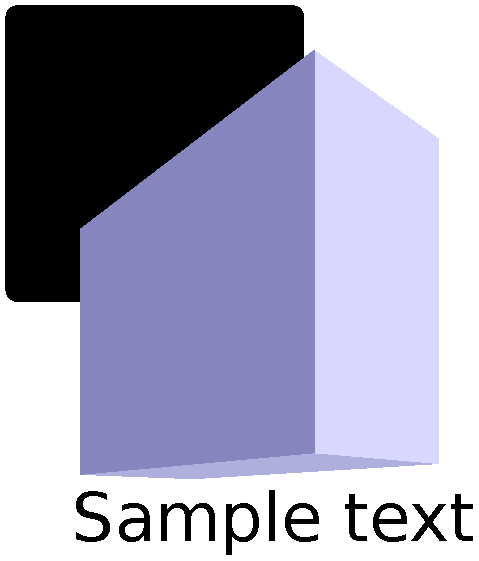
\includegraphics[width=0.3\linewidth]{fig1.pdf}
  \caption{Пример работы программы}
  \label{fig:prog-ex}
\end{figure}


\begin{equation}
  \label{eq:f1}
  E=mc^2,
\end{equation}

\noindent{}где $m$ -- это масса, $c$ -- скорость света в вакууме, \ldots

Новый абзац. Рассмотрим формулу (\ref{eq:f1}).


\chapter*{ЗАКЛЮЧЕНИЕ}

В таблице~\ref{tbl:ex} представлены результаты сравнения производительности\ldots

\begin{table}[hb]
  \caption{Пример таблицы}\label{tbl:ex}
  \centering
\begin{tabularx}{1\textwidth} {
  | >{\raggedright\arraybackslash}X
  | >{\centering\arraybackslash}X
  | >{\raggedleft\arraybackslash}X | }
 \hline
 item 11 & item 12 & item 13 \\
 \hline
 item 21  & item 22  & item 23  \\
\hline
\end{tabularx}
\end{table}

\begin{thebibliography}{99}
\bibitem{bratko90} И.~Братко. Язык программирования Пролог для искусственного интеллекта. М\;:~Наука. 1990. 310~c.
\bibitem{b2} DeRidder J.L. The immediate prospects for the application of ontologies in digital libraries // Knowledge Organization -- 2007. -- Vol. 34, No. 4. P.~227-246.
\bibitem{b2}  U.S. National Library of Medicine. Fact sheet: UMLS Metathesaurus\;:\;[текст]~/ National Institutes of Health, 2006-2013. -- URL:
\url{http://www.nlm.nih.gov/pubs/factsheets/umlsmeta.html} (дата обращения: 2014-12-09).
\bibitem{b2}  U.S. National Library of Medicine. Fact sheet: Unfied Medical Language System\;:\;[текст]~/ National Institutes of Health, 2006--2013. -- URL:\url{http://www.nlm.nih.gov/pubs/factsheets/umls.html} (дата обращения: 2009-12-09).
\bibitem{b3}  Антопольский А.Б., Белоозеров В.Н. Процедура формирования макротезауруса политематических информационных систем // Классификация и кодирование. -- 1976. -- N 1 (57). -- С.~25--29.
\bibitem{b4}  Белоозеров В.Н., Федосимов В.И. Место макротезауруса в лингвистическом обеспечении сети органов научнотехнической информации // Проблемы информационных систем. -- 1986. -- N 1. -- С.~6--10.
\bibitem{b5}  Использование и ведение макротезауруса ГАСНТИ:Методические рекомендации / ГКНТСССР -- М., 1983. -- 12~с.
\bibitem{b6}  Nuovo soggettario: guidaalsistemaitaliano di indicizzazione per soggetto, prototipo del thesaurus\;:\;[рецензия]~// Knowledge Organization. -- 2007. -- Vol. 34, N 1. -- P.~58--60.
\bibitem{b7}  ГОСТ 7.25-2001 СИБИД. Тезаурус информационно-поисковый одноязычный. Правила разработки, структура, состав и форма представления. -- М., 2002. -- 16~с.
\bibitem{b8}  Nanoscale Science and Technology Supplement: Collection ofapplicable terms fromPACS 2008\;:\;[текст]~// PACS 2010 Regular Eddition /~AIP Publishing. -- URL: \url{http://www.aip.org/publishing/pacs/nano-supplement} (дата обращения: 2014-12-09).
\bibitem{b9}  Смирнова О.В. Методикасоставления индексов УДК // Научно-техническая информация. Сер.~1. -- 2008. -- N 8. -- С.~7--8.
\bibitem{b10}  Индексирование фундаментальных научных направлений кодами информационных классификаций УДК /~О.А.~Антошкова, Т.С.~Астахова, В.Н.~Белоозеров и др.; под ред.акад. Ю.М.~Арского. -- М., 2010. -- 322~с.
\bibitem{b11}  Рубрикатор как инструмент информационной навигации /~Р.С.~Гиляревский, А.В.~Шапкин, В.Н.~Белоозеров. - СПб.\;: Профессия, 2008. -- 352~с.
\bibitem{b12}  Рубрикатор научно-технической информации по нанотехнологиям и наноматериалам / РНЦ "Курчатовский институт",
ФГУ ГНИИ ИТТ "Информика", Национальный электронно-информационный консорциум (НЭИКОН), Всероссийский институт научной и технической информации (ВИНИТИРАН). -- М., 2009. -- 75~с.
\bibitem{b13}  Рубрикатор по нанонауке и нанотехнологиям\;:\;[сайт]~-- URL:\url{http/www.rubric.neicon.ru} (дата обращения: 12-02-2022)
\end{thebibliography}

\appendices

\chapter{Исходный код программ}
\chapter{Документация разработчика}

\end{document}




%%% Local Variables:
%%% mode: latex
%%% TeX-master: t
%%% End:
